% Copyright 2022 Edoardo Riggio

% Licensed under the Apache License, Version 2.0 (the "License");
% you may not use this file except in compliance with the License.
% You may obtain a copy of the License at

% 	http://www.apache.org/licenses/LICENSE-2.0

% Unless required by applicable law or agreed to in writing, software
% distributed under the License is distributed on an "AS IS" BASIS,
% WITHOUT WARRANTIES OR CONDITIONS OF ANY KIND, either express or implied.
% See the License for the specific language governing permissions and
% limitations under the License.

\documentclass{article}

\usepackage{hyperref, amsmath, graphicx, amssymb, csquotes, tabularx}
\usepackage{fancyvrb,newverbs,xcolor}

\graphicspath{ {./assets/} }

\definecolor{cverbbg}{gray}{0.93}

\newenvironment{cverbatim}
 {\SaveVerbatim{cverb}}
 {\endSaveVerbatim
  \flushleft\fboxrule=0pt\fboxsep=.5em
  \colorbox{cverbbg}{\BUseVerbatim{cverb}}%
  \endflushleft
}

\newenvironment{lcverbatim}
 {\SaveVerbatim{cverb}}
 {\endSaveVerbatim
  \flushleft\fboxrule=0pt\fboxsep=.5em
  \colorbox{cverbbg}{%
    \makebox[\dimexpr\linewidth-2\fboxsep][l]{\BUseVerbatim{cverb}}%
  }
  \endflushleft
}

\newcommand{\ctexttt}[1]{\colorbox{cverbbg}{\texttt{#1}}}
\newverbcommand{\cverb}
  {\setbox\verbbox\hbox\bgroup}
  {\egroup\colorbox{cverbbg}{\box\verbbox}}

\begin{document}
\begin{titlepage}
    \begin{center}
        \vspace*{1cm}
        
        \Huge
        \textbf{Distributed Systems Cheatsheet}
        
        \vspace{0.5cm}
        \LARGE
        
        \vspace{.5cm}
        
        Edoardo Riggio
   		  \vspace{1.5cm}
       
        \vfill
        
        \today
        
        \vspace{.8cm}
          \Large
          Distributed Systems - S.A. 2022 \\
        Software and Data Engineering \\
        Universit\`{a} della Svizzera Italiana, Lugano \\
        
    \end{center}
\end{titlepage}

\tableofcontents

\newpage

\section{Introduction}
With the advent in the mid 1980's of 16-, 32-, and 64-bit CPUs -- as well as the invention of high-speed computer networks, made it possible for the creation of large numbers of geographically-dispersed networks of computers. These are known as \textbf{distributed systems}.

\subsection{Definition}
A distributed system is a collection of independent computers that appear to the user as a single coherent system. \\ \\
Each computing element of these massive systems are able to behave independently from one another. A computing element is often referred to as a \textbf{node}. This node can either be a hardware device or a software process.

\subsection{Consequences}
Some of the main negative consequences that arise when dealing with distributed systems are the following:

\begin{itemize}
	\item \textbf{Concurrency} \\
	This happens when several processes try to read and write on a shared storage service.
	
	\item \textbf{Absence of a global clock} \\
	Each node will have its own notion of time. This means that there is no common reference of time between the nodes.
	
	\item \textbf{Failure independency}
	The failure of a node can make another node unusable.
	
\end{itemize}

\subsection{Challenges}
Some of the challenges that arise when dealing with distributed systems are outlined in the following sections.

\subsubsection{Openness}
The services are offered according to standard rules. These rules describe both the syntax and semantics of such services. The standard rules of distributed systems are called \textbf{COBRA}(Common Object Request Broker Architecture).

\subsubsection{Scalability}
Scalability can be with respect to the \textbf{system size} -- which would mean adding more users to the system; to the \textbf{geography} -- which would deal with users lying far apart from one another; and to \textbf{administration} -- which would deal with the complexity to manage an increasing system. \\ \\
Some scalability techniques are the following:

\begin{itemize}
	\item \textbf{Hiding communication latencies} \\
	This is important for \textbf{geographical scalability}. Asynchronous communications can be used to reduce the waiting time of the users. This can be achieved with the use of batch processing and parallel applications.
	
	\item \textbf{Distribution} \\
	Components are split into parts and spread across the system. An example of this would be the DNS, where we have a tree of domains divided into non-overlapping zones. Furthermore, the name in a zone is handled by a single name service.
	
	\item \textbf{Replication} \\
	This can be use to increase both \textbf{availability} and \textbf{performance}, as well as reduce \textbf{latency}. Moreover, caching can be used as a form of replication, but is typically done on-demand.
\end{itemize}

\subsubsection{Transparency}
Transparency is the ability of a system to hide some of its characteristics or errors to the user. There exist several different forms of transparency:

\begin{itemize}
	\item \textbf{Access transparency} \\
	Hide the differences in data representation and machine architecture.
	
	\item \textbf{Location transparency} \\
	Users cannot tell where a resource is physically located.
	
	\item \textbf{Relocation transparency} \\
	Even if the entire service was moved from one data center to the other, the user wouldn't be able to tell.
	
	\item \textbf{Migration transparency} \\
	Moving processes and resources initiated by users, without affecting any ongoing communication and operation.
	
	\item \textbf{Replication transparency} \\
	Hide the existence of multiple replicas of one resource.
	
	\item \textbf{Concurrency transparency} \\
	Each user is not going to notice if another user is making use of the same resource.
	
	\item \textbf{Failure transparency} \\
	The user or application does not notice that some piece of the system fails to work properly. The system is then able to automatically recover from the failure.
\end{itemize}

\subsection{Types of Distributed Systems}
There are three main types of distributed systems: \textbf{distributed computing systems}, \textbf{distributed information systems}, and \textbf{distributed pervasive systems}.

\subsubsection{Distributed Computing Systems}
These systems aim at high-performance computing tasks. These systems can be part of two subtypes:

\begin{itemize}
	\item \textbf{Cluster Computing} \\
	All the resourced are located in a local-area network, and are using the same OS. In addition, they also have a common administrative domain.
	
	\item \textbf{Grid Computing} \\
	This is a "federation" of computer systems. Such systems may have different administrative domains, different hardware, software... Such systems are used to make collaboration between organisations feasible.
\end{itemize}

\subsubsection{Distributed Information Systems}
These systems are based on transactions. These transactions are used to make systems communicate between themselves. Transactions follow the \textbf{ACID} properties:

\begin{itemize}
	\item \textbf{Availability} \\
	To the user, the transaction happens indivisibly.
	
	\item \textbf{Consistency} \\
	The transaction does not violate system invariants.
	
	\item \textbf{Isolation} \\
	Concurrent transactions do not interfere with each other.
	
	\item \textbf{Durability} \\
	Once a transaction commits, the changes are permanent.
\end{itemize}

\noindent The application components of each node communicate directly with each other.

\subsubsection{Distributed Pervasive Systems}
These systems are composed by mobile and embedded computing devices. This means that pervasive systems need to have the following characteristics:

\begin{itemize}
	\item Embrace contextual changes
	\item Encourage ad-hoc composition
	\item Recognise sharing as the default
\end{itemize}

\noindent Some examples of such architectures are home systems, electronic health care systems, and sensor networks.

\section{Architectures}
In a distributed system there are two types of architectures:

\begin{itemize}
	\item \textbf{Software Architectures} \\
	How software components are organised and interact between each other.
	
	\item \textbf{System Architectures} \\
	How software components are instantiated on real machines.
\end{itemize}

\subsection{Software Architectures}
Software architectures are based on \textbf{components}, which are modular units with well-defined interfaces. Software architectures can be of several different types:

\begin{itemize}
	\item \textbf{Layered architectures}
	\item \textbf{Object-based architectures}
	\item \textbf{Data-centred architectures}
	\item \textbf{Event-based architectures}
\end{itemize}

\subsubsection{Layered Architectures}
In this kind of architecture, the components at layer $L_i$ can call components in layer $L_{i-1}$, but not components in layer $L_{i+1}$.

\begin{center}
	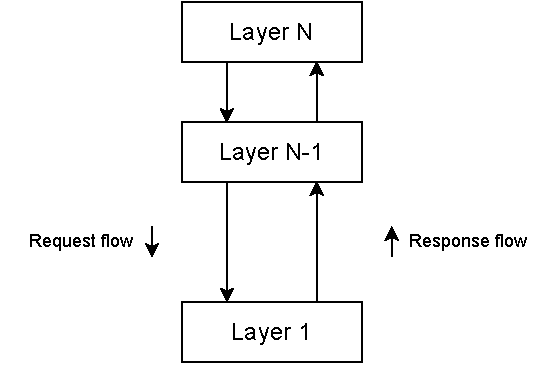
\includegraphics[width=7cm, height=5cm, keepaspectratio]{assets/layered.pdf}
\end{center}

\subsubsection{Object-Based Architectures}
Each object is a component connected through a remote procedure call mechanism.

\begin{center}
	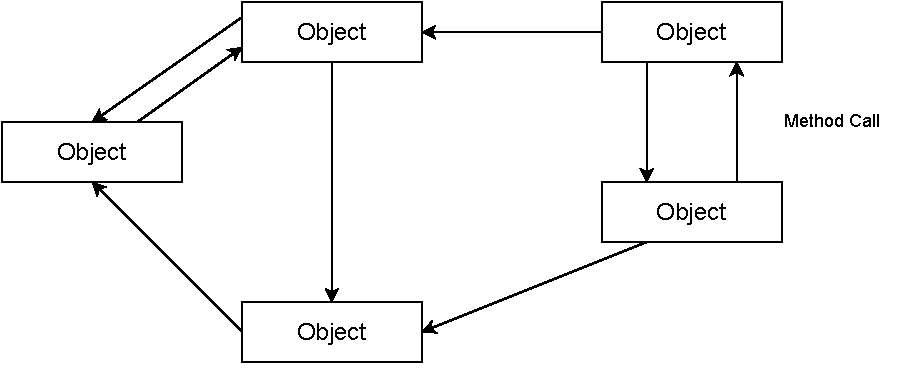
\includegraphics[width=11cm, height=5cm, keepaspectratio]{assets/object-based.pdf}
\end{center}

\subsubsection{Data-Centred Architectures}
The processes communicate through a common repository. This repository can be, for example, a shared distributed file system or a database.

\begin{center}
	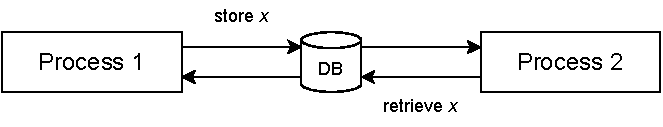
\includegraphics[width=8cm, height=5cm, keepaspectratio]{assets/data-centered.pdf}
\end{center}

\subsubsection{Event-Based Architectures}
The processes communicate through the propagation of events (\textbf{publish-subscribe system}). The middleware ensures that the process which subscribes to that events will receive them. \\ \\
Processes are loosely coupled, this means that they do not to refer to each other.

\begin{center}
	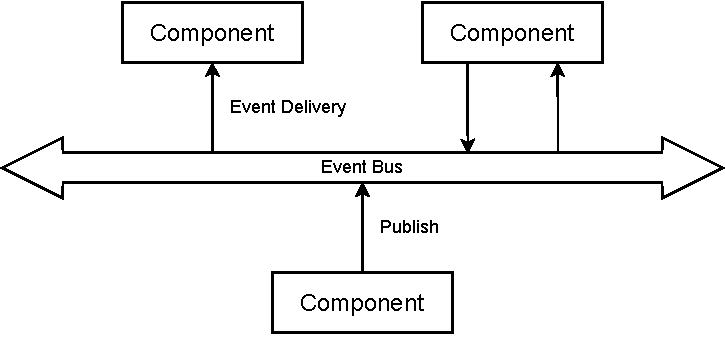
\includegraphics[width=9cm, height=5cm, keepaspectratio]{assets/event-based.pdf}
\end{center}

\subsubsection{Shared Data-Space Architecture}
These architectures are similar to data-centred and event-based architectures.

\begin{center}
	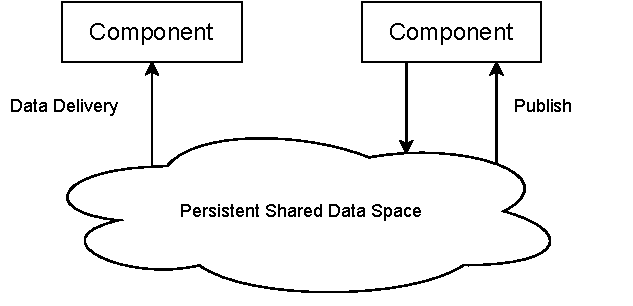
\includegraphics[width=8cm, height=5cm, keepaspectratio]{assets/shared.pdf}
\end{center}

\subsection{System Architectures}
System Architectures describe what software components are used, where to place each component, and how the components interact with each other. \\ \\
There are two types of system architectures:

\begin{itemize}
	\item \textbf{Centralised architectures}
	\item \textbf{Decentralised architectures}
\end{itemize}

\subsection{Centralised Architecture}
Centralised architectures follow the Client-Server model. The \textbf{server} implements some services, while the \textbf{client} requests services and waits for replies. \\ \\
The communication between server and client is \textbf{connectionless}. This means that it is highly efficient, but it is more complex to handle transmission failures (UDP). \\ \\
Server and client may also use another way to communicate. This protocol is connection-oriented, relatively low performance, but more reliable. This is because the node makes a request and receives a reply back in the same connection. \\ \\
Centralised architectures can be either \textbf{single-} or \textbf{multi-layered}. Multi-layered architectures enable to divide concerns, meaning that clients can contain only the program implementing the user-interface level (or only part of it). Moreover, architectures can also be \textbf{multi-tiered}.

\subsection{Decentralised Architectures}
Decentralised architectures can be either vertically or horizontally distributed.

\begin{itemize}
	\item \textbf{Vertical Distribution} \\
	It can be achieved by placing logically different components on different machines. An example of this is a three-tiered application.
	
	\item \textbf{Horizontal Distribution} \\
	Both clients and servers are physically split up into logically equivalent parts. Each part operates on its own share of the dataset. An example of this is a peer-to-peer system.
\end{itemize}

\subsubsection{Structured Peer-to-Peer Architectures}
Structured peer-to-peer architectures are deterministic procedures used to build an \textbf{overlay network}. Here nodes are processes, and links are possible communication channels. \\ \\
In the case of a structured peer-to-peer architecture, we use \textbf{Distributed Hash Tables} (DHT). Each data item that is maintained by the system, is uniquely associated with a key, and this key is subsequently used as an index. Moreover, to each node of the system is assigned an identifier. Each node is made responsible for storing data associated with a specific subset of keys. \\ \\
Any node can be asked to look up a given key, which boils down to efficiently routing that lookup request to the node responsible for storing the data associated with the given key. \\ \\
An example of a structural peer-to-peer architecture is a \textbf{Chord}, which is depicted below.

\begin{center}
	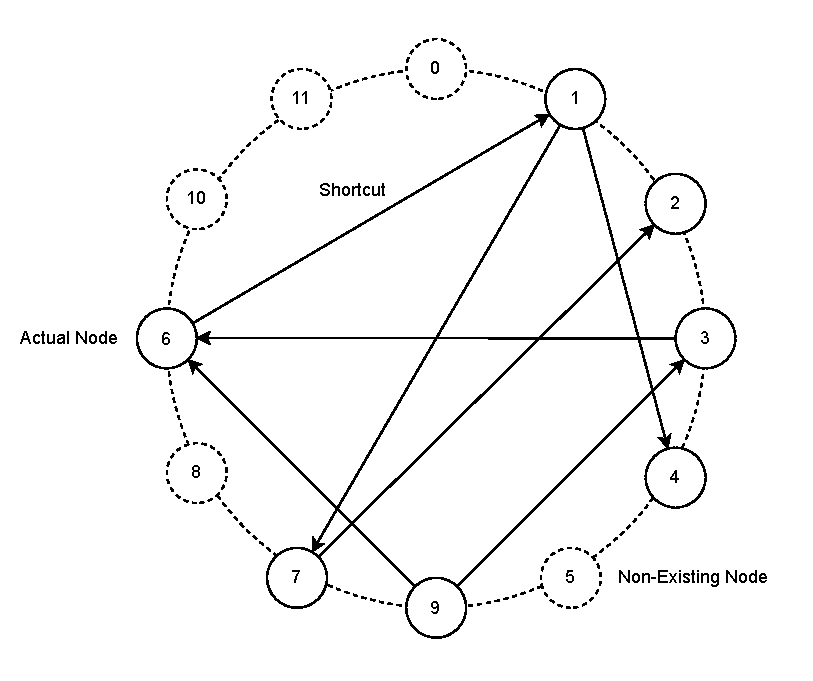
\includegraphics[width=12cm, height=9.5cm, keepaspectratio]{assets/chord.pdf}
\end{center}

\subsubsection{Unstructured Peer-to-Peer Architectures}
In this type of architecture, the overlay network is built using a randomised procedure. Each node in the network has a list of neighbours, constructed in a random way. This results in a random graph. \\ \\
In these kinds of systems, when a node joins the network, it often contacts a well-known node to obtain a starting list of other peers in the system. Moreover, the nodes generally change their local list almost continuously. \\ \\
Unlike in structured peer-to-peer architectures, looking up data cannot follow a predetermined route. Instead, in this case we need to resort to searching for data. This can be done in different ways, such as \textbf{flooding}, \textbf{random walks}, or \textbf{policy-based} search methods.

\begin{center}
	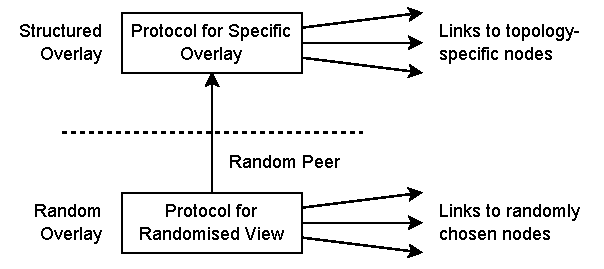
\includegraphics[width=8cm, height=5cm, keepaspectratio]{assets/unstructured.pdf}
\end{center}

\subsection{Super Peer}
\textbf{Brokers} are services that collect data on resource usage and availability for a number of nodes that are in each other's proximity. This allows to quickly select the node with sufficient resources. \\ \\
Nodes that act as brokers are called \textbf{super peers}. Super peers organise themselves into a structured peer-to-peer network, leading to a hierarchical organisation of nodes. The nodes that connect to these super peers are known as \textbf{weak peers}.

\begin{center}
	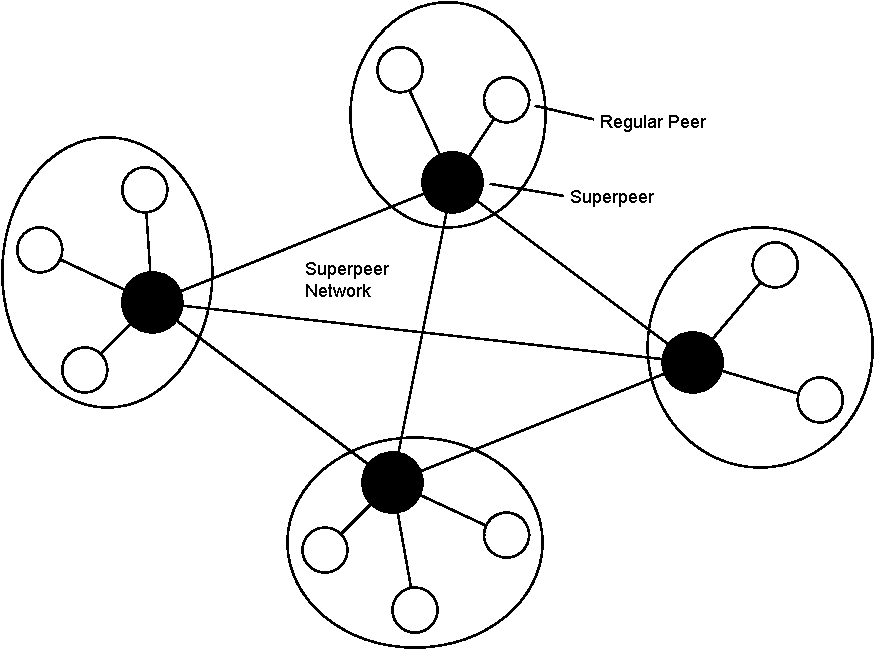
\includegraphics[width=9cm, height=10cm, keepaspectratio]{assets/superpeer.pdf}
\end{center}

\subsection{Middleware}
Middleware provides a degree of distribution transparency. They can either follow an object-based architectural style, or an event-based architectural style.

\subsubsection{Interceptors}
They offer a means to adapt the middleware. Interceptors break the usual flow of control and allow other application-specific code to be executed. Moreover, they are used to improve software management.

\subsubsection{Wrappers and Adapters}
Wrappers and adapters provide a similar interface to the original abstraction, and implement additional logic before or after invoking the original interface.

\subsubsection{Proxies and Stubs}
They provide -- as in the case of wrappers and adapters -- a similar interface as the original abstraction. However, in this case proxies and stubs usually own components rather than extending previously defined ones.

\section{Processes}
\subsection{Introduction}
Virtual processors are created by the OS. A process is a program executed on one of these virtual processors. Each processor has a process table in which several different values relative to the process are stored. \\ \\
Concurrent processes are protected from each other by making the sharing of CPU and hardware resources transparent and using special hardware. \\ \\
Every time a new process is created, the OS must create an independent address space as well. This is known as \textbf{context switching}, and it's really expensive.

\subsection{Threads}
A thread is a lightweight process that can run inside of a process. Threads share the same memory space. For this reason, context switching between threads is less expensive than between processes. \\ \\
Threads are used in distributed systems mainly for making communication calls non blocking. \\ \\
In the case of servers with \textbf{single-threaded models}, one thread receives the request and executes it rapidly. This is known as sequential processing. \\ \\
On the other hand, in the case of servers with \textbf{finite state machine models}, one thread executes the requests and the replies. Blocking system calls are replaced by non-blocking ones, and multiple requests can be handled in parallel.

\subsection{Virtualisation}
The role of virtualisation -- in distributed systems -- is to extend or replace existing interfaces and mimic the behaviour of other systems. \\ \\
The main reasons of virtualisation are the following:

\begin{itemize}
	\item Allow legacy software to run on new mainframe hardware
	\item Porting legacy interfaces to new platforms
	\item Isolating systems running on the same server
\end{itemize}

\subsection{Superservers}
A superserver is a kind of server that listens on many ports and fork a process to execute a service.

\subsection{Stateless vs Stateful Servers}
A server is said to be \textbf{stateless} if it does not keep any information about the state of the client. \\ \\
On the other hand, a server is said to be \textbf{stateful} if it maintains persistent information about the clients. This solution is better in terms of performance (it caches data of the users), but can be problematic in the case that the server crashes or experience other memory-related issues.

\subsection{Server Clusters}
A server cluster is a collection of machines connected through a network. Such clusters have three tiers:

\begin{enumerate}
	\item \textbf{Logical Switch} \\
	It receives client requests and route them to the servers.
	
	\item \textbf{Application Servers} \\
	Low-end servers are used when the storage is the bottleneck of the system. Otherwise, high-end servers are used when the service deals with computationally expensive computations.
	
	\item \textbf{Data-Processing Servers} \\
	The databases.
\end{enumerate}

\section{Communication}
In layered protocols, process \textit{A} con communicate with process \textit{B} by building a message in its address space. After doing so, a system call is used to send the message from \textit{A} to \textit{B}.

\subsection{OSI Model}
The \textbf{Open System Interconnection} (OSI) \textbf{Reference Model} is an ISO standard. This type of model is never widely used or implemented. \\ \\
The OSI model makes use of connection-oriented protocols. Both the sender and the receiver explicitly establish a connection, they communicate, and finally explicitly terminate the connection. \\ \\
The OSI model is divided into the following parts:

\begin{itemize}
	\item Application layer
	\item Presentation layer
	\item Session layer
	\item Transport layer
	\item Network layer
	\item Data link layer
	\item Physical layer
\end{itemize}

\noindent In the following sections, we will have a bottom-up look at the different layers.

\subsubsection{Physical Layer}
This layer deals with how to send bits from one end to the other. It standardises electrical, mechanical, and signalling interfaces. finally, it does not handle errors.

\subsubsection{Data Link Layer}
The data link layer groups the bits into frames and ensures their correct transmission. It uses checksums to verify the integrity of the data frames.

\subsubsection{Network Layer}
It routes the messages from source to destination. To do so, it needs a routing protocol. The most common ones are:

\begin{itemize}
	\item \textbf{TCP} \\
	Transmission Control Protocol (TCP) is both reliable and connection-oriented.
	
	\item \textbf{UDP} \\
	Universal Datagram Protocol (UDP) is both unreliable and connectionless.
\end{itemize}

\subsubsection{Session Layer}
The session layer is an enhanced version of the transport layer -- but rarely supported.

\subsubsection{Presentation Layer}
This layer simplifies the communication between machines with different internal data representation.

\subsection{Middleware Protocols}
This type of protocols usually resides at the application layer. The middleware protocols can have several different roles, such as:

\begin{itemize}
	\item Authentication
	\item Commit protocols
	\item Distributed locking protocols
\end{itemize}

\subsection{Types of Communication}
There are several different ways in which a client and a server can communicate:

\begin{itemize}
	\item \textbf{Persistent Communication} \\
	The message is stored by the communication middleware until it can be delivered to the receiver.
	
	\item \textbf{Transient Communication} \\
	The message is delivered only if both sender and receiver are executing.
	
	\item \textbf{Asynchronous Communication} \\
	The sender continues immediately after submitting the message. This message is temporarily stored inside of the middleware.
	
	\item \textbf{Synchronous Communication} \\
	the server is blocked until the message has been received by the receiver.
\end{itemize}

\subsection{Remote Procedure Call}
A \textbf{Remote Procedure Call} (RPC) is a simple communication mechanism, and is more natural than the send/receive primitives.

\subsubsection{Basic RPC Operation}
The RPC first makes itself look like a local procedure call. When a read operation is performed, a client stub is called. The client stub pack all the parameters into a message and sends it to the server. \\ \\
Both the calling and the receiving procedures are not aware of the distribution of the system.

\subsection{Message-Oriented Communication}
Message-oriented transient communication uses \textbf{Berkeley sockets}. These sockets are communication endpoints used by applications to read are write. The process of the socket is the following: \\ \\
Server:

\begin{enumerate}
	\item Create the socket
	\item Bind the socket to a port
	\item Listen on the opened port
	\item Accept upon communication request
	\item Communicate with the client
	\item Close the socket
\end{enumerate}

\noindent Client:

\begin{enumerate}
	\item Create the socket
	\item Request connection to the server
	\item Communicate with the server
	\item Close the socket
\end{enumerate}

\subsubsection{Message-Queuing Models}
The applications communicate between one another by inserting messages into queues. Each application has its own private queue, and both the sender and receiver do not have to necessarily be active at the same time. \\ \\
There is guarantee of delivery at destination, but the time at which it reaches its destination cannot be known. \\ \\
Queue managers interact with both relays and applications. The relays forward the messages to other queue managers. The message is delivered as follows:

\begin{enumerate}
	\item Queue managers interact with both application and relays
	\item The relays forward the messages to other queue managers
	\item The overlay network composes the sender, the destination, and the relays
\end{enumerate}

\subsubsection{Message Brokers}
A message broker acts as an application-level gateway. They do so by integrating existing and new applications into a single coherent system. Moreover, they convert the incoming messages ti formats that can be understood by the destination application.

\subsection{Multicast Communication}
Application-level multicasting has the following characteristics:

\begin{itemize}
	\item Support for sending data to multiple receivers
	\item Nodes reorganise themselves into an overlay network at the application level
\end{itemize}

\noindent There are two main types of overlays:

\begin{itemize}
	\item \textbf{Tree-Based Overlay} \\
	There is a single path between every pair of nodes.
	
	\item \textbf{Mesh-Based Overlay} \\
	There are multiple paths between every two pair of nodes. Although it is harder to find the best path between a pair of nodes, these overlay networks are generally more robust.
\end{itemize}

\section{Naming}
It is impossible to memorise IPv4 and IPv6 addresses to reach websites. For this reason. we use \textbf{naming}. Naming can be of three types:

\begin{itemize}
	\item Flat
	\item Structured
	\item Attribute-Based
\end{itemize}

\subsection{Flat Naming}
Flat names are composed of names, identifiers, and addresses. They can be described as follows:

\begin{itemize}
	\item \textbf{Name} \\
	It is "human-friendly" and it is not necessarily unique or used for identifying.
	
	\item \textbf{Identifier} \\
	It uniquely identifies an entity.
	
	\item \textbf{Address} \\
	It is not "human-friendly" and is used for low-level naming of access points.
\end{itemize}

\subsubsection{Forwarding Pointers}
When an entity is moved from point \textit{A} to point \textit{B}, it leaves a reference in point \textit{A} pointing to \textit{B}. The requests to \textit{A} must be forwarded to \textit{B} in a transparent manner. \\ \\
There are some drawback to forwarding:

\begin{itemize}
	\item Fast moving entities leave a long chain of entities
	\item Each intermediate location needs to allocate resources for the forwarding process
	\item Any missing step in the chain makes the whole chain unusable
\end{itemize}

\subsubsection{Home-Based Approaches}
In this case, a home location is used to keep track of the current location. By doing so, IPv6 addresses become identifiers. The following is the procedure of home-based approaches:

\begin{enumerate}
	\item Mobile devices requests a local temporary address
	\item The address is registered with the home agent
	\item The home agent forwards the packets to the mobile device
	\item The home agent tells the sender the new temporary location
\end{enumerate}

\noindent There are some drawbacks that come with home-based approaches, such as:

\begin{itemize}
	\item Increased latency
	\item Home agent must always be available
	\item Permanent relocations must be handled
\end{itemize}

\noindent A possible solution to all of these problems comes with registering home locations using a \textbf{Domain Name Server} (DNS).

\subsubsection{Distributed Hash Tables}
We assign an \textit{m}-bit identifier space to each node of the system. To resolve the successor node \textit{k}, we use a \textbf{finger table}.

\[ FT_p[i] = succ(p + 2^{i-1}) \]

\noindent Where \textit{p} is the node, and \textit{i} is the number of nodes succeeding \textit{p}. The complexity of the successor computation is:

\[ O(\log (nodes)) \]

\noindent A drawback of this method is that nodes joining and leaving force the finger table to continuously update. This issue can be solved by making the nodes run the function \verb|succ(k)| in the background.

\subsubsection{Hierarchical Approaches}
Each \textbf{root node} keeps track only of the location of the directory nodes of the next lower-level subdomains. On the other hand, each \textbf{leaf node} contains the location of the entities. \\ \\
A lookup request is performed bottom-up. This means that the request is forwarded amongst the children of the directory node. Afterwards, the request goes up the hierarchy.

\subsection{Structured Naming}
\subsubsection{Name Spaces}
Name spaces can be represented as labeled, directed graphs with directory and leaf nodes. \\ \\
A \textbf{pathname} is a sequence of labels corresponding to the edges in that path.

\subsubsection{Linking and Mounting}
A \textbf{symbolic link} is a link between a node and an absolute path. This is particular since normally nodes are linked to files -- in the case of a OS's file system. \\ \\
Mounting a foreign name space in a distributed system is a type of symbolic link. For this symbolic link to work it requires:

\begin{itemize}
	\item Name of an access protocol
	\item Name of a server
	\item Name of the mounting point in the foreign name space
\end{itemize}

\subsubsection{Name Space Distribution}
Generally, large-scale name services are organised into \textbf{organisational layers}. The layers are the following:

\begin{itemize}
	\item \textbf{Global Layer} \\
	It is composed by the root name and its children (very stable)
	
	\item \textbf{Administrational Layer} \\
	The nodes are managed by a single organisation (somewhat stable)
	
	\item \textbf{Managerial Layer} \\
	Nodes are managed locally (may change frequently)
\end{itemize}

\subsubsection{Name Resolution}
All clients have access to a name resolver. This name resolution can happen in two ways:

\begin{itemize}
	\item \textbf{Iteratively} \\
	The name resolver performs each step of the name resolution.
	
	\item \textbf{Recursively} \\
	The name resolver delegates the name resolution to the root server.  
\end{itemize}

\noindent Each one of the previously described methods has its own drawbacks. In the case of the \textbf{iterative} method, it has high communication costs and poor caching capabilities. In the case of the \textbf{recursive} method, it has an increased load on each server of the chain, as well as increased latency for non-cached requests.

\subsubsection{DNS Name Space}
The DNS is a hierarchically organised name space. Some of its characteristics are:

\begin{itemize}
	\item DNS root has no name
	\item Each subtree is a domain
	\item The path to the subtree root node is the domain name
	\item All nodes contain records
	\item One server is responsible for one zone
\end{itemize}

\subsection{Attribute-Based Naming}
Attribute-based naming systems are also known as directory services. In this case, an entity is described in terms of an \verb|(attribute, value)| pair. A set of these attributes is used for searching.

\subsubsection{LDAP}
\textbf{Lightweight Directory Access Protocol} (LDAP) has the following characteristics:

\begin{itemize}
	\item Each service contains a number of directory entries
	\item Each entry is composed of a number of \verb|(attribute, value)| pairs
	\item Each attribute has an associated type
	\item Attributes can be single- or multi-valued
	\item The collection of all entries for a service is called a \textbf{Directory Information Base} (DIB)
\end{itemize}

\noindent In a DIB, each entry has a \textbf{Relative Distinguished Name} (RDN). This name is globally unique. \\ \\
RDNs can be used a globally unique names -- which is the same thing that happens in DNS. Moreover, the RDNs establish a hierarchy of entries -- which is known as the \textbf{Directory Information Tree} (DIT).

\end{document}



































